\documentclass{article}
\usepackage{tikz}
\usepackage{geometry}
\geometry{%
  paperwidth=9.72cm,
  paperheight=10.76cm,
  margin=5mm
}
\begin{document}


\section{Introduction}

\begin{tikzpicture}[line width=0.5mm]
  \draw (0,0) -- (1,1);
\end{tikzpicture}

\tikz[line width=0.5mm]{\draw (0,0) -- (1,1);}

\section{Especificación de puntos}
\begin{center}
  \begin{tikzpicture}
    \draw (0,0) circle (1pt);
    \draw (5mm,1cm) circle (1pt);
    \draw[red] (5mm,-1cm) circle (1pt);
    \draw (0,0) -- (2,2);
  \end{tikzpicture}
\end{center}

\begin{center}
  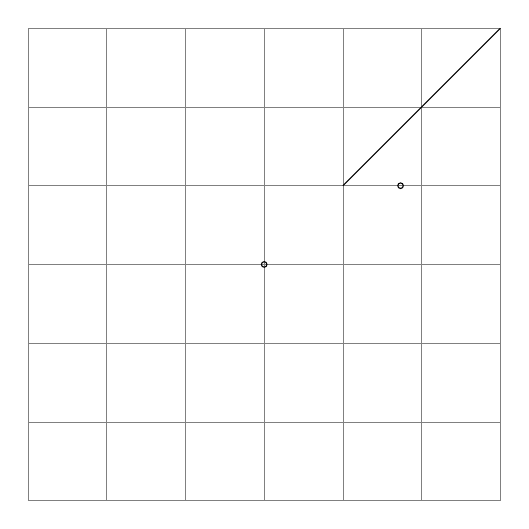
\begin{tikzpicture}
    \draw[help lines] (-3,-3) grid (3,3);
    \draw (30:2cm) circle (1pt);
    \draw (0,0) circle (1pt);
    \draw (1,1) -- ++(2,2);
  \end{tikzpicture}
\end{center}

\section{Trazado de serie de líneas}
\begin{center}
  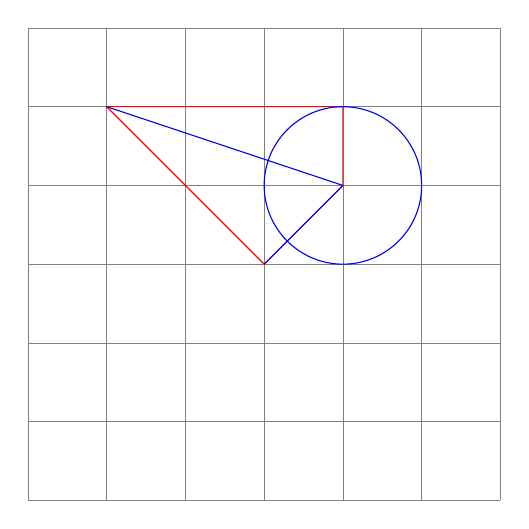
\begin{tikzpicture}
    \draw[help lines] (-3,-3) grid (3,3);
    \draw[red] (0,0) -- (1,1) -- (1,2) -- (-2,2) -- cycle;
    \draw[blue] (0,0) -- (1,1) circle (1) -- (-2,2) -- cycle;
  \end{tikzpicture}
\end{center}

\section{Acciones con caminos o paths}
\begin{center}
  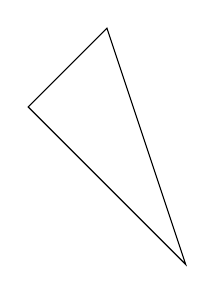
\begin{tikzpicture}
    \path[draw] (0,0) -- (1,1) -- (2,-2) -- cycle;
  \end{tikzpicture}
\end{center}

\begin{center}
  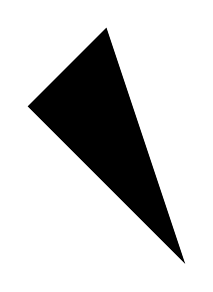
\begin{tikzpicture}
    \path[fill] (0,0) -- (1,1) -- (2,-2) -- cycle;
  \end{tikzpicture}
\end{center}

\begin{center}
  
\begin{tikzpicture}
    \path[shade] (0,0) -- (1,1) -- (2,-2) -- cycle;
  \end{tikzpicture}
\end{center}

\begin{center}
  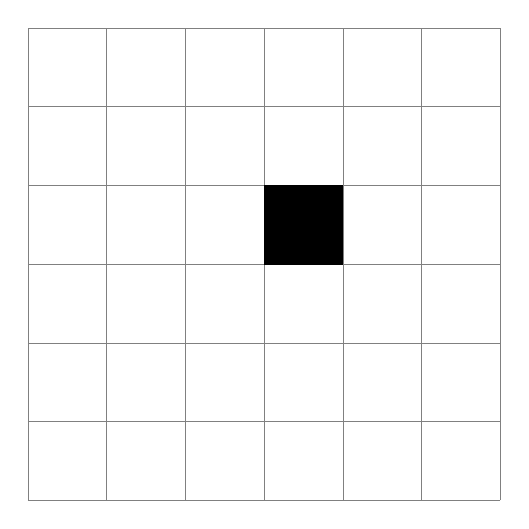
\begin{tikzpicture}
    \draw[help lines] (-3,-3) grid (3,3);
    \path[clip] (0,0) -- (1,0) -- (1,1) -- (0,1) -- cycle;
    \path[fill] (-1,-1) -- (2,-1) -- (2,2) -- (-1,2) -- cycle;
  \end{tikzpicture}
\end{center}






\end{document}



